\documentclass[14pt]{beamer}
\usepackage{graphicx}
\graphicspath{ {./images/} }

\title{MaskifAI}
\subtitle{A mask detection web app}
\author[TEAM 6]{Sachita Malhotra, Shruthi Rao, Srishti Negi}
\date{June 2020}


\usetheme{AnnArbor}

\newcounter{saveenumerate}
\newcommand{\saveenumerate}{\setcounter{saveenumerate}{\value{enumi}}}
\newcommand{\restartenumerate}{\setcounter{enumi}{\value{saveenumerate}}}

\begin{document}

\begin{frame}
    \titlepage
\end{frame}

\begin{frame}
    \frametitle{Where would you feel safer?}
    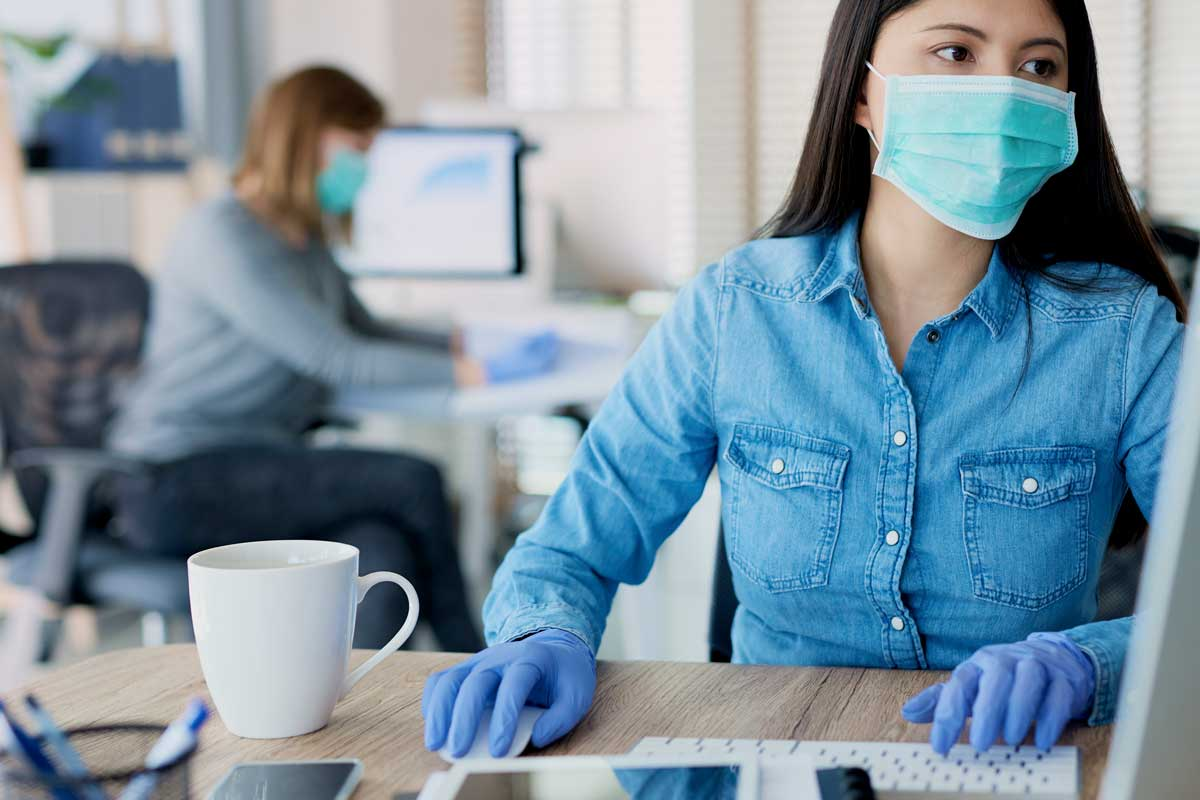
\includegraphics[width=4.5 cm,height=3.5 cm]{office_mask}
    \includegraphics[width=4.5 cm,height=3.5 cm]{no_office_mask}
\end{frame}

\begin{frame}
    \frametitle{Overview}
    Our project aims to create a mask detection web application which can be used by organizations to ensure that everybody who enters the workspace wears a mask.
\end{frame}

\begin{frame}
    \frametitle{Mask Detection}
    \begin {figure}
        \begin{minipage}{0.5\textwidth}
            \centering
            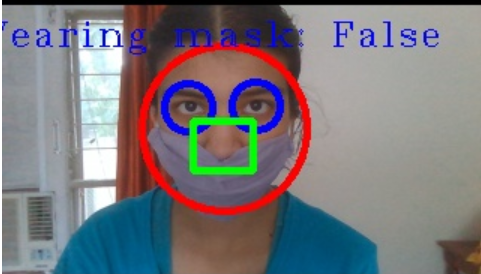
\includegraphics[width=3.5 cm,height=2.5 cm]{a}
            \caption{First}
        \end{minipage}
        \pause[2]
        \begin{minipage}{0.5\textwidth}
            \centering
            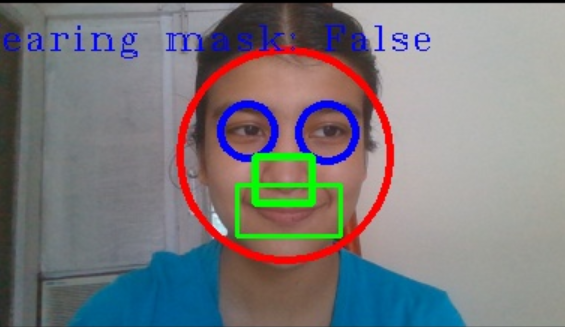
\includegraphics[width=3.5 cm,height=2.5 cm]{b}
            \caption{Second}
        \end{minipage}%
        \pause[3]%
        \begin{minipage}{0.5\textwidth}
            \centering
            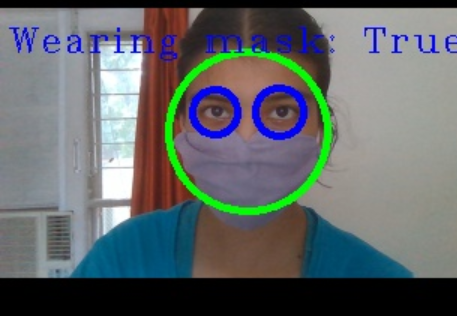
\includegraphics[width=3.5 cm,height=2.5 cm]{c}
            \caption{Third}
        \end{minipage}
    \end{figure}
\end{frame}

\begin{frame}
    \frametitle{Tech Stack}
    \begin{enumerate}
        \item OpenCV
        \item Flask
        \item SQLite
        \item HTML
        \item CSS
    \end{enumerate}
\end{frame} 

\begin{frame}
    \frametitle{Description}
    At the entrance
    \begin{enumerate}
        \item The website would be running in a system at the entrance

        \item Employees: Log into the application to check if ze is wearing a mask properly

        \item Mask not detected: Manager notified
    \end{enumerate}
\end{frame}

\begin{frame}
    \frametitle{Description}
    At employee's workspace
    \begin{enumerate}
        \item Provides periodic sanitization notifications to employee
            
        \item General hygiene and precautions for Covid-19 information
    \end{enumerate}
\end{frame}

\begin{frame}
    \frametitle{Target Audience}
    The web application is  aimed at helping organizations take precautions against Covid-19 by ensuring that all the employees who enter the workspace wear masks.
\end{frame}

\begin{frame}
    \frametitle{Status}
    \begin{enumerate}
        \item Implemented mask detection in local system
        \item Improved mask detection accuracy
        \item Made a web app - login and mask detction
        \item Working on the notification feature
    \end{enumerate}
\end{frame}

\begin{frame}
    \frametitle{Learnings and Challenges}
    Learnings:
    \begin{enumerate}
        \item Using pre-trained classifiers to implement feature detection
        \item How to use Flask extensions to implement-
        \begin{enumerate}
            \item Login feature
            \item Database
            \item Store encrypted data using werkzeug.security
        \end{enumerate}
    \end{enumerate}
    Challenges:
    \begin{enumerate}
        \item Integration of mask detection script with database
        \item Web push nofication
    \end{enumerate}
\end{frame}

\begin{frame}
    \frametitle{References}
    \begin{enumerate}
        \item OpenCV documentation: https://opencv.org/
        \item Flask documentation: https://flask.palletsprojects.com/en/1.1.x/
        \item A comparison of face and facial feature detectors based on the Viola-Jones general object detection framework: https://link.springer.com/article/10.1007/s00138-010-0250-7
    \end{enumerate}
\end{frame}

\end{document}
